\documentclass[12pt,a4paper,oneside]{book}
\usepackage{lmodern}
\usepackage[svgnames]{xcolor} % Required to specify font color
\input{../LaTexTemplate/templates/couleurs.tex}
\usepackage{makeidx}
\usepackage[utf8]{inputenc} 
\usepackage{marvosym}
\usepackage[T1]{fontenc}
\usepackage[francais]{babel}
\usepackage[top=1.7cm, bottom=1.7cm, left=1.7cm, right=1.7cm]{geometry}
\usepackage{verbatim}
\usepackage[urlbordercolor={1 1 1}, linkbordercolor={1 1 1}, linkcolor=vert1, urlcolor=bleu, colorlinks=true]{hyperref}
\usepackage{tikz} %Vectoriel
\usepackage{listings}
\usepackage{fancyhdr}
\usepackage{multido}
\usepackage{amssymb}
\usepackage{float}
\usepackage[francais]{minitoc}
\usepackage[final]{pdfpages} 
\usepackage{pgfgantt}
\usepackage{graphicx} % Required for box manipulation
\usepackage{makeidx}
\usepackage{lscape}
\usepackage{rotating}
\usepackage{epstopdf}


\newcommand{\titre}{Documentation de BandStorm}
\newcommand{\logoFooter}{~}
\newcommand{\logo}{mdl.png}
\newcommand{\titreFooter}{Documentation -- BandStorm} 
\newcommand{\subtitle}{\textbf{I}ntégration, \textbf{V}érification, \textbf{V}alidation, \textbf{Q}ualification} 
\newcommand{\auteur}{%
}
\newcommand{\semestre}{S9}
\newcommand{\annee}{2015}
\newcommand{\pole}{}
\newcommand{\formation}{}
\newcommand{\sigle}{}

\makeindex

\input{../LaTexTemplate/templates/listings.tex}
\input{../LaTexTemplate/templates/classroomsTemplates/l3/cours.tex}
\input{../LaTexTemplate/templates/remarquesExempleAttention.tex}
\input{../LaTexTemplate/templates/polices.tex}
\input{../LaTexTemplate/templates/affichageChapitre.tex}
\input{../LaTexTemplate/templates/cover/couverture.tex}
\makeatother


\begin{document}
	\thispagestyle{empty} % Removes page numbers
	\titleBC

	\setcounter{tocdepth}{1}
	\setcounter{secnumdepth}{3}
	\setcounter{minitocdepth}{1}
	
	\tableofcontents
	\chapter{Le projet}
	\section{Le projet Bandstorm}
	Bandstorm est un projet qui a pour but de réaliser un réseau social pour des amateurs de musique. Celui-ci a pour objectif de mettre en relations des utilisateurs par le biais de communautés. Ces communautés sont constitués en fonction de préférences musicales.

%Heroku + Logins
%Sonar
%Github + github utilisateur
	\section{Les informations utiles\ldots}
	\subsection{Github}
	\begin{description}
		\item[Lien du dépôt] \url{https://github.com/BandStormTeam/BandStormProject}~\\
		\item[Liens vers les profils]~
			\begin{description}
				\item[Steve Magras] \url{https://github.com/smagras}
				\item[Zaccaria Zyat] \url{https://github.com/SirAbel}
				\item[Antoine de Roquemaurel] \url{https://github.com/aroquemaurel}
				\item[Julian Bironneau] \url{https://github.com/johnSilver7}
				\item[Dylan Roletto] \url{https://github.com/vlaks} 
			\end{description}
	\end{description}

	\subsection{Intégration et déploiement continue}
	\begin{description}
		\item[Travis-CI] \url{https://travis-ci.org/BandStormTeam/BandStormProject }
		\item[Heroku] \url{https://m2dl-bandstorm.herokuapp.com/}~\\
			\begin{exemple}
				Il est possible de se connecter avec l'utilisateur merry et le mot de passe password.
			\end{exemple}
	\end{description}

	\subsection{Qualité du code}
	\begin{description}
		\item[Coveralls] \url{https://coveralls.io/github/BandStormTeam/BandStormProject}
		\item[SonarQube] \url{http://sonar.joohoo.fr/dashboard/index/BandStormProject}~\\
			\begin{attention}
				\textbf{Attention}, le serveur sonar n'est pas disponible 24/24. Il est accessible entre 10h et 23h.
			\end{attention}
	\end{description}


	\section{Fonctionnalités}
	Notre application possède de multiples fonctionnalités qui vont être détaillées ci-dessous.
	Chaque utilisateur de BandStorm possède un compte personnel sécurisé par un système de login.
	
	\begin{itemize}
		\item Les utilisateurs ont la possibilité de suivre d’autres utilisateurs.
		\item Les utilisateurs peuvent créer, rejoindre et visualiser un groupe.
		\item Les utilisateurs peuvent créer et visualiser un évênement.
		\item Les utilisateurs ont la possibilité de rechercher des entités via une barre de recherche (utilisateurs, groupes, évênements).
		\item Les utilisateurs peuvent poster des statuts.
		\item Les utilisateurs peuvent visualiser les statuts de leurs abonnements.
		\item Les utilisateurs ont la possibilité de “lighter” (aimer) un statut.
		\item Les utilisateurs ont la possibilité de changer leurs informations personnelles.
	\end{itemize}	
	
	\chapter{Le \textit{workflow} de développement}
	Afin de faciliter le travail collaboratif et l'intégration de nos développements respectifs, nous avons utilisé Git et Github. 
	Via un \textit{workflow} en branches par fonctionnalités, nous avons pu développer celles-ci en parallèles. 
	
	Lorsqu'un développeur choisi de répondre à une issue, il va créer une nouvelle branche, nommée suivant la convention suivante
	\texttt{sprintN/noIssue-recapitulatifIssue}.
	
	Lorsque le développeur estime avoir terminé sa fonctionnalité, il ouvre une \textit{Pull Request}, celle-ci nous permet d'effectuer de la revue de code. La fonctionnalité ne sera fusionnée avec la branche de niveau inférieur que lorsque l'équipe estime avoir terminé l'issue.
	\begin{figure}[H]
		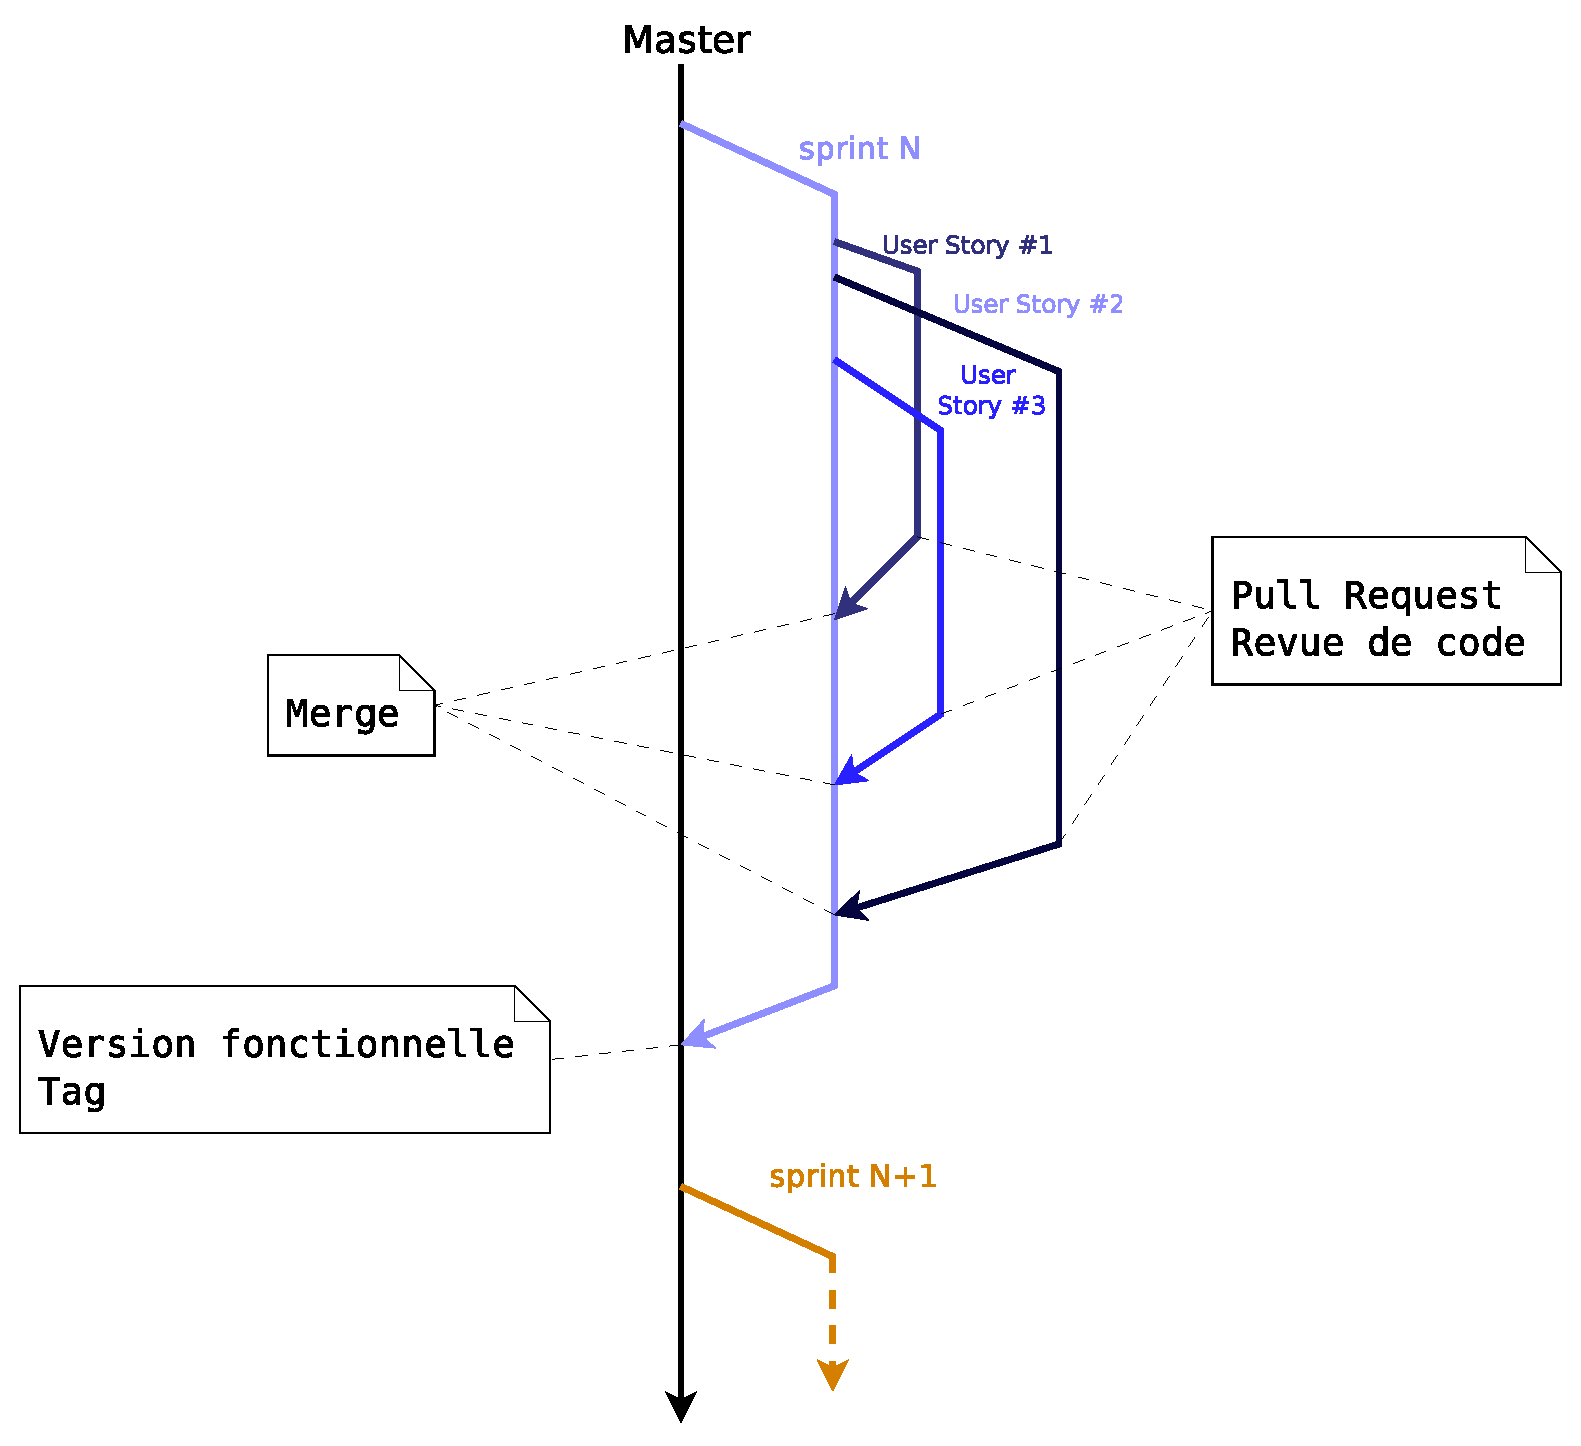
\includegraphics[width=15.5cm]{../beamer/images/Process/BranchingWorkflow.eps}
		\caption{\textit{Workflow} en \textit{feature} branches}
	\end{figure}
	Plus de détails notre \textit{workflow} est disponible ici
	: \newline
	\url{https://github.com/BandStormTeam/BandStormProject/blob/master/workflow-feature.md}
	
	\section{Tests et couverture}
	Lors du développement d'un projet complexe, il est indispensable de tester correctement le projet afin de pouvoir le vérifier et le valider. Ainsi, dans le cadre de BandStorm nous avons définis des pourcentages de couverture de tests à respecter impérativement; Le bon respect de ces chiffres contribuent à effectuer un projet de qualité. 
	
	Cette couverture doit être de 80\% en ligne de code, 
	\begin{itemize}
		\item 100\% pour les classes du domaine.
		\item 80\% pour les contrôleurs.
		\item 80\% pour les services.
	\end{itemize}	
	
	Les classes du domaine, services et contrôleurs devront être couverts par des tests unitaires. Les services de type DAO devront être couverts par des tests d'intégrations.
	
	Afin d’avoir des tests les plus exhaustifs possibles, nous avons également mis en place des tests fonctionnels en utilisant Geb. Ces tests nous permettent de vérifier le bon fonctionnement global de notre application.
	
	\section{Intégration continue}
	Nous avons utilisés Travis-CI afin d’intégrer et de vérifier cette intégration de manière continue. Notre serveur d’intégration effectue plusieurs actions : 
	\begin{itemize}
		\item Compilation du projet 
		\item Lancement des tests unitaires
		\item Lancement des tests d’intégration
		\item Calcul de la couverture de code
		\item Éventuel déploiement sur heroku (uniquement master)
	\end{itemize}
	Le build ne peut être correcte que si l'ensemble de ces actions se sont bien effectuées. 

	\begin{exemple}
	À noter que Travis CI ne lance pas les tests fonctionnels. En effet, les tests fonctionnels nécessitent un serveur graphique
	ainsi que le démarrage d’un navigateur. Travis-CI propose une aleternative pour simuler un environnement graphique, mais
	celui-ci ne semble pas fonctionner avec Geb. Il pourrait être intéressant d'installer un serveur d’intégration continue sur une
	machine personnelle tel que Jenkins ou Gitlab-CI, nous n'aurions pas cette limite de serveur X.
	\end{exemple}

	Les tests fonctionnels étant les tests les plus proches d’un utilisateur permettrait ainsi de pouvoir effectuer de la non-régression de façon systématique et automatique.
	
	\section{Déploiement continue}
	La vérification de la bonne intégration de notre application ne suffit pas à avoir un processus de mise en production fiable. Il est indispensable de vérifier le bon déploiement de l'application sur un serveur autre que celui de production. C'est dans ce but que nous utilisons Heroku. La La branche master de l'application est déployée de façon continue et automatique.
	
	\section{Analyse statique de code}
	Pour avoir un code de qualité, il est faut également prendre en compte la maintenance que celui-ci va couter. Cette maintenance peut être réduite en développant avec des conventions claires précises et mesurables. 
	Ainsi, nous avons utilisé codenarc qui permet de vérifier les règles de nos conventions d’écritures. 
	
	SonarQube quant à lui permet d’une part de centraliser toutes les informations nécessaires, tout en conservant un historique de celles-ci, mais il nous permet également d’avoir de nouvelles métriques tel que le nombre de ligne de code, le pourcentage de commentaire ou la complexité cyclomatique de notre projet. 
	
	\chapter{Agilité}
	\section{Sprints}	
	Pendant toutes la durée du projet, l’équipe à suivi les principes du processus agile Scrum. La durée du projet a été découpée en trois sprints d’une durée de deux semaines chacun. Un sprint 0 a été réalisé afin de mettre en place l’architecture, le processus de développement et la première version du Backlog.
	
	Il a été décidé que la répartition des rôles de \textit{Product owner }et de \textit{Scrum Master }changent à chaque Sprint afin que tout le monde puisse essayer chacun des roles.
	
	Une revue et une rétrospective ont été effectuées à la fin de chaque Sprint.\\
	Le tableau ci-dessous recense les différents sprints associés aux rôles et aux date de revues et rétrospectives.

	\hspace{-40px}
	\begin{tabular}{|c|c|c|c|}
		\hline
		& \textbf{Sprint 1 }& \textbf{Sprint 2 }& \textbf{Sprint 3}\\
		\hline
		Dates & 30/09/2015 $\rightarrow$ 13/10/2015 & 14/10/2015 $\rightarrow$ 27/10/2015 & 28/10/2015 $\rightarrow$ 11/11/2015\\
		\hline
		Product Owner & Julian Bironneau &Dylan Roletto& Zaccaria Zyat\\
		\hline
		Scrum Master & Steve Magras & Antoine de Roquemaurel &Julian Bironneau\\
		\hline
		Dates revues & 14/10/2015& 28/10/2015& 12/11/2015\\
		\hline
		Dates rétrospectives & 14/10/2015& 28/10/2015 &12/11/2015 \\
		\hline
	\end{tabular}
	
	\section{Planning Poker et vélocité}
	Pour attribuer un nombre de points aux issues, l'équipe a effectué des planning poker. Ceci au travers d'un outil disponible
	gratuitement sur internet, \textit{Pointing Poker}\newline (\url{https://www.pointingpoker.com/}).
	
	Après avoir terminé un sprint, il nous était donc possible de calculer la vélocité de celui-ci. Le plugin ZenHub nous a permis de représenter facilement et de manière graphique la courbe Burn-Down de notre vélocité. 
	
	Ci-dessous, le burn-down représentant le premier sprint:
	\begin{figure}[H]
		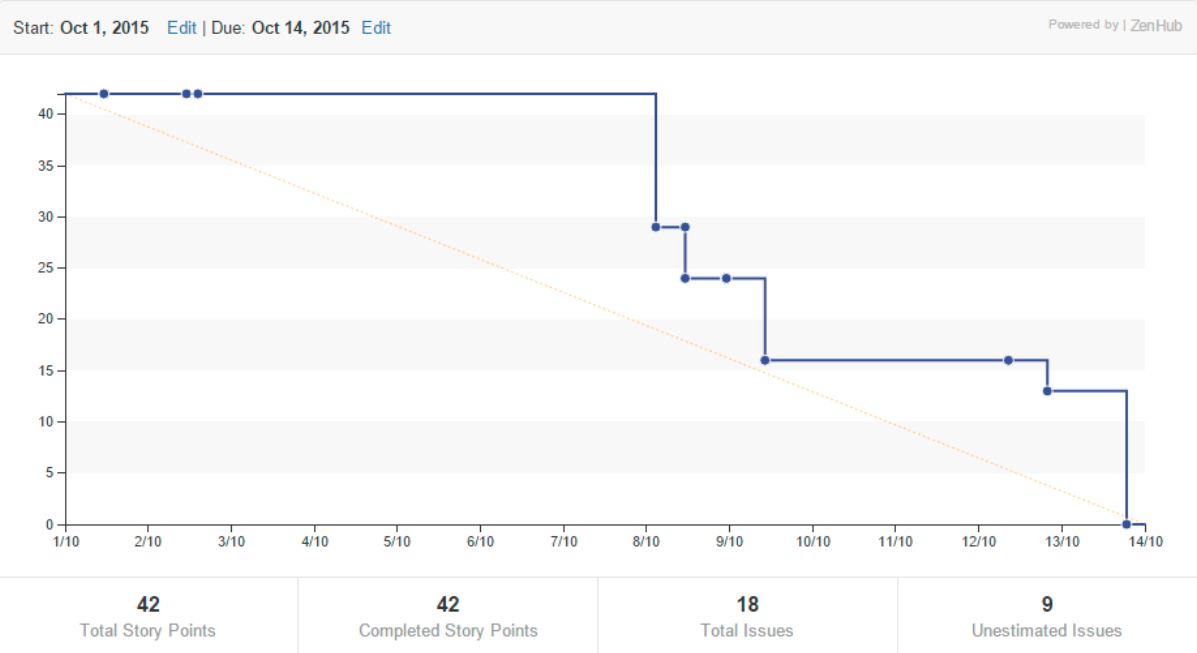
\includegraphics[width=18cm]{../beamer/images/Results/methodo/burndown.png}
		\caption{Burndown chart du premier Sprint}
	\end{figure}
	Les résultats obtenus pour la vélocité de ce projet sont indiqués dans le tableau ci-dessous:

	\begin{tabular}{|c|c|c|c|}
		\hline
		\textbf{Sprint} &\textbf{ Points prévus} & \textbf{Points effectués }&\textbf{ Nombre d'issues}\\
		\hline
		Sprint 1, v0.1 &42& 42& 18\\
		\hline
		Sprint 2, v0.2 &44& 44& 13\\
		\hline
		Sprint 3, v1.0 &23& 20& 15\\
		\hline
	\end{tabular}
	\section{Objectifs des sprints}
	Les sprints ont été guidés par les objectifs de sprints ci-dessous:

\begin{description}
	\item[Sprint 1] Avoir les fonctionnalités basiques d’identification d’un réseau social. 
	\item[Sprint 2] Permettre aux membres de bandstorm de pouvoir intéragir sur le site.
	\item[Sprint 3] Corriger les bogues et de rajouter des fonctionnalités d'intéractions entre les utilisateurs. 
\end{description}

	\section{Définition de fini}
	On détermine qu'un \textit{user stories} est terminée lorsque : 

	\begin{itemize}
		\item Les tests unitaires et d’intégrations sont passés
		\item 100\% de couverture de code pour les classes du modèle
		\item 80\% de couverture de code pour les classes controleurs
		\item 80\% de couverture de code pour les classes services et dao
		\item Les tests d’acceptation sont passés
		\item La pull request est revue par le product owner
		\item Le build est passé sur Travis CI
		\item Les critères codenarc sont respectés 
		\item Correction des criticals et majors sur SonarQube
		\item La javadoc est rédigée 
	\end{itemize}

	\section{Releases}
	Après avoir effectué les trois sprints, une release a été plannifée. Cette release est le résultat de tous les travaux
	effectués au cours du projet. Le projet doit être livré à Franck Silvestre le 12/11/2015 et être déployé sur le serveur Heroku.

	\chapter{Architecture}
	Bandstorm s'appuyant sur le framework grails, une grande partie de l'architecture et de l'organisation est structurée par
	celui-ci. Ainsi, nous utilisons le modèle MVC, c'est-à-dire la séparation des contrôleurs vis-à-vis des vues HTML et des
	modèles. 

	Ci-dessous est disponible le diagramme de classes des modèles de notre application.
	\begin{figure}[H]
		\hspace{-33px}
		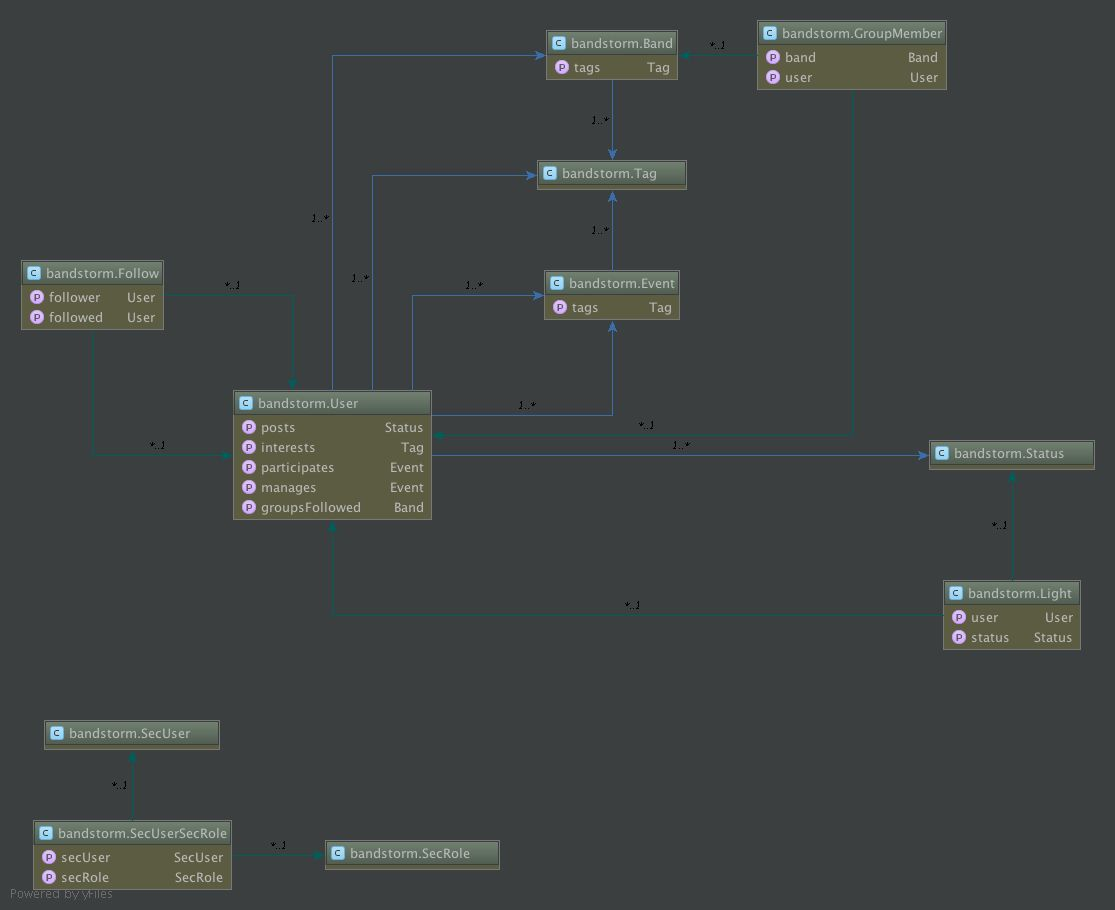
\includegraphics[width=20cm]{classes.png}
		\caption{Diagramme de classe de BandStorm}
	\end{figure}
\end{document}
